\section{Introduction}
\label{sec:introduction}

This review concerns the non-centrosymmetric barium yttrium zinc silicate $\mathrm{Ba_5Y_{12}Zn[O(SiO_4)]_8}$. We pursue three questions: whether the composition and structural assignment of the target phase can be confirmed; under which phase-formation conditions the phase can be obtained reproducibly; and whether a continuous composition--structure relationship connects the Zn-containing phase to the Zn-free tetragonal Ba--Y silicates. In the original report, crystals were grown from a high-temperature solution in an open system and the structure was solved by single-crystal X-ray diffraction (SCXRD)~\cite{ababaikeri2024ba5y12zn}. The structure combines a framework of highly coordinated rare-earth--oxygen polyhedra with isolated or composite silicate units, and it offers a reference point both for how complex silicates assemble and for the compositional design of non-centrosymmetric oxides.

The direct report of the target phase establishes only that the crystals exist and what their structure is; it gives no independently reproducible starting composition, no phase-formation range, and no route to phase-pure bulk samples~\cite{ababaikeri2024ba5y12zn}. We therefore do not stitch together a ``best recipe'' from the conditions used for structurally related compounds. Instead, we separate the questions that single-crystal growth, solid-state reaction, and phase-diagram screening can each answer, and we use that separation to design experiments that discriminate between alternative structural hypotheses. Literature values are quoted throughout with their stated limitations; structurally related systems and process-reference systems serve only to suggest experimental reference points.

\subsection{Current Understanding of Related Systems}

\paragraph{The tetragonal Ba--Y--Si--O silicate family.}
Early flux-growth experiments reported $\mathrm{Ba_{5+x}Y_{13}Si_8O_{41}}$ as an accompanying crystalline phase, and a later series of 151 runs in the BaO--K$_2$O--Y$_2$O$_3$--SiO$_2$--MoO$_3$ system showed that the Y$_2$O$_3$\slash SiO$_2$ ratio, the MoO$_3$ content, and the cooling rate together govern which silicate structure type forms and how well the crystals grow~\cite{kolitsch2009crystal,wierzbickawieczorek2017high}. Recent single-crystal work has recast the related nominal composition as non-stoichiometric $\mathrm{Ba_xY_{26}Si_{16}O_{71+x}}$, and ceramic experiments showed that grinding in agate can introduce SiO$_2$ and push bulk samples off the nominal ratio~\cite{yamane2024synthesis,yamane2024microstructure}. A separate phase-region study that combined energy-dispersive spectroscopy (EDS), continuous rotation electron diffraction (cRED), synchrotron powder X-ray diffraction (PXRD), and neutron diffraction confirmed $\mathrm{Ba_5Y_{13}[SiO_4]_8O_{8.5}}$ and found competing phases and a glass-forming region~\cite{gulay2024navigation}. Taken together, these results place the target phase inside a phase region governed jointly by the Ba\slash Y\slash Si ratio, oxygen stoichiometry, liquid composition, and thermal history, not at the end of a single isolated recipe.

\paragraph{Structurally related Ba--Zn--Si--O compounds.}
Ba$M$SiO$_4$ ($M$~=~Co, Zn, Mg) belongs to the family of stuffed-tridymite derivatives, which shows that divalent tetrahedral cations can replace one another within a given framework; it does not follow that these structures are isostructural with the Y-containing target phase~\cite{liu1993structures}. The low- and high-temperature forms of BaZn$_2$Si$_2$O$_7$ can be told apart by neutron and X-ray diffraction, a reminder that the observation temperature and the cooling path both bear on structure assignment~\cite{lin1999phase}. A solid-state study of BaZnSi$_3$O$_8$ proceeded through calcination, pelletizing, sintering, and controlled cooling, with characterization by synchrotron or laboratory X-ray diffraction~\cite{zou2021crystal}. The main lesson of the Ba--Zn--Si--O literature is therefore to record the Zn source, the atmosphere, the cooling path, and the phases present at both high temperature and room temperature together, rather than to borrow any single temperature outright.

\paragraph{Y--Si--O process-reference systems.}
Y$_2$SiO$_5$ and Y$_2$Si$_2$O$_7$ each occur in several polymorphs and have been prepared by high-temperature solution growth, melt growth, and the Czochralski method. Diffraction, local spectroscopy, and high-temperature measurements show that each polymorph, and the product that remains after cooling, must be identified separately~\cite{redhammer2003beta,becerro2004revisiting,dolan2008structures,pang2005study}. These studies help standardize how crucible, flux, volatilization loss, slow cooling, and annealing conditions are recorded, but they do not show that the same growth methods apply to $\mathrm{Ba_5Y_{12}Zn[O(SiO_4)]_8}$.

\subsection{Organization of the Review}

We first verify the literature sources for the target phase and its structural relatives, then summarize what earlier experiments have established about composition, competing phases, contamination, and thermal history, then compare the synthesis routes and their experimental conditions, and finally propose four research directions: a local phase diagram, Zn--Y--oxygen-stoichiometry coupling, solid-state reaction run in parallel with high-temperature solution growth, and Mg\slash Co analogs. The two-step inorganic retrosynthesis model used here generates only a set of precursors to be tested; temperatures, atmospheres, crucibles, and characterization methods are still fixed from the literature and from materials-chemistry constraints.

Figure~\ref{fig:research-roadmap} summarizes the line of argument. Related systems are used first to establish structural relationships, competing phases, and process boundaries; phase-diagram and charge-balance analysis then proposes candidate compositions, from which the retrosynthesis model derives the precursor set; solid-state reaction and high-temperature solution growth test the bulk phase region and the single-crystal structure, respectively; and composition and process are adjusted round by round on the basis of the phase composition, the measured stoichiometry, and the structure refinement. Each round of experiments should eliminate at least one structural or phase-region hypothesis rather than chase an unverified ``best recipe''.

\begin{figure*}[t]
  \centering
  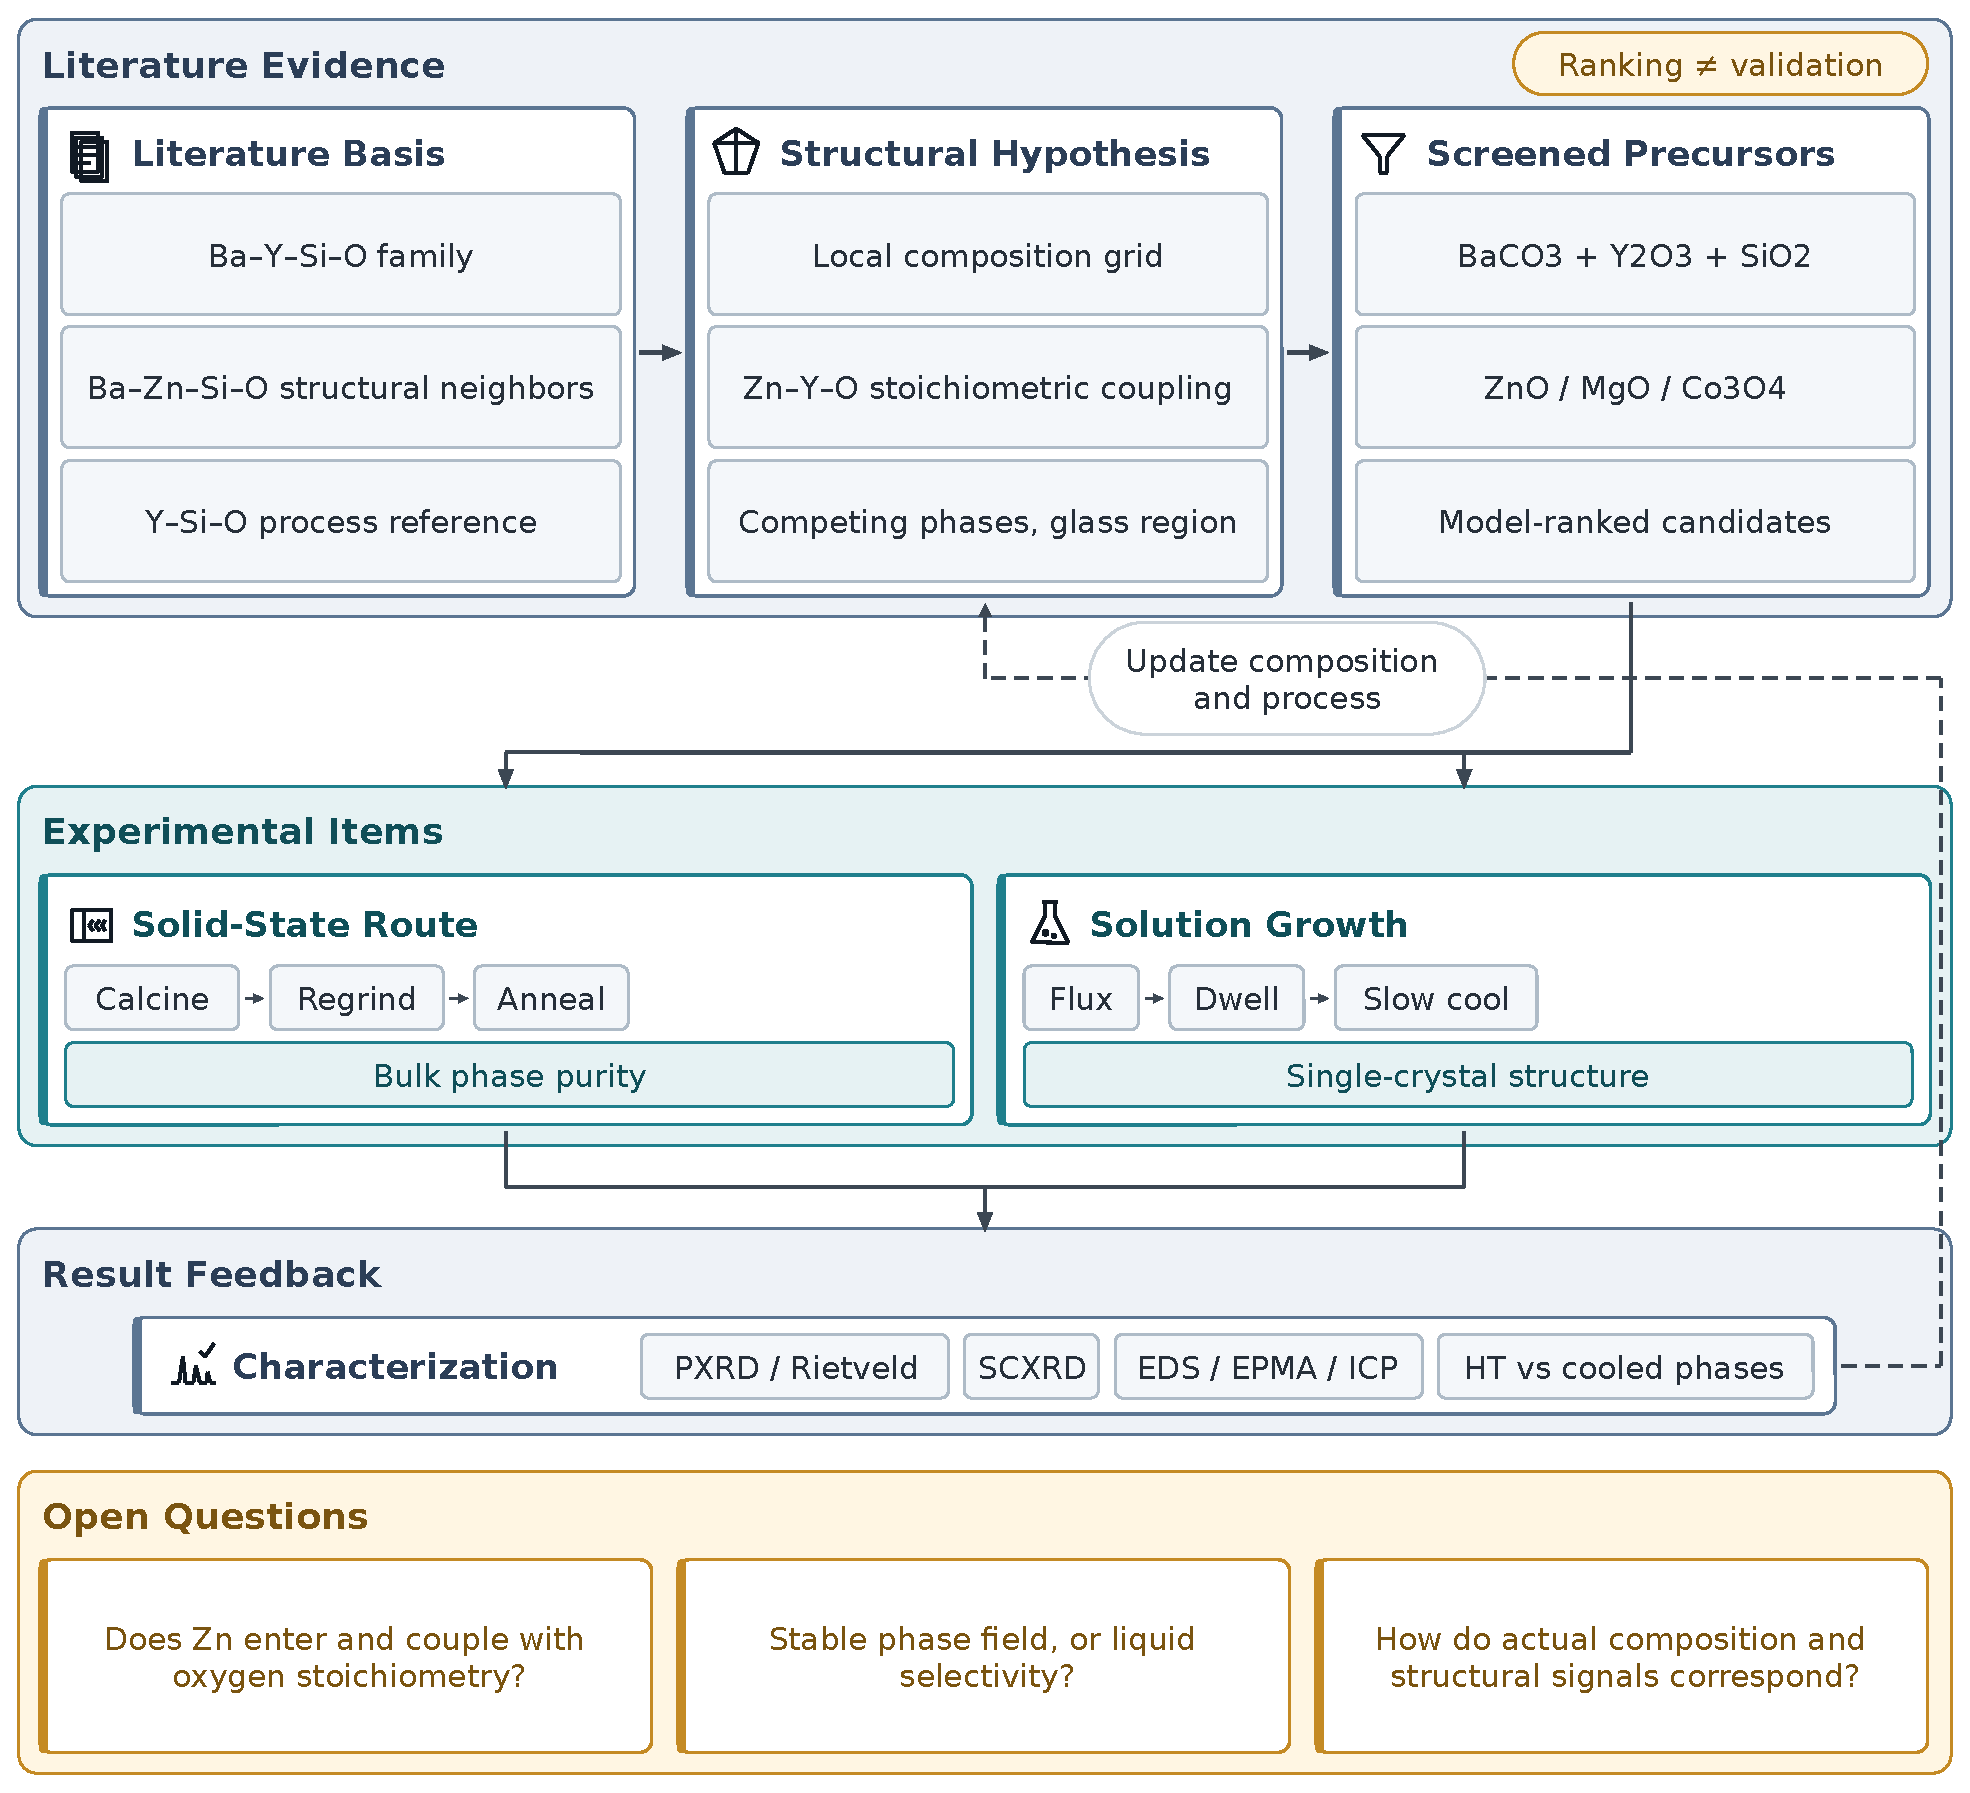
\includegraphics[width=\textwidth]{../figures/pdf/fig03_research_roadmap_en.pdf}
  \caption{\textbf{Research roadmap.} The Ba--Y--Si--O, Ba--Zn--Si--O, and Y--Si--O systems are used first to establish structural relationships, competing phases, and process boundaries; phase-diagram and charge-balance analysis proposes candidate compositions, and the two-step inorganic retrosynthesis model supplies the precursor set; solid-state reaction and high-temperature solution growth probe the bulk phase region and the single-crystal structure, respectively, and the characterization results feed back into the next round of compositions and processes.}
  \label{fig:research-roadmap}
\end{figure*}
